\documentclass{article}
\usepackage[utf8]{inputenc}
\usepackage{natbib}
\usepackage{graphicx}
\usepackage{geometry}
\usepackage[T1]{fontenc}
\geometry{ margin=1.3in}
\usepackage{enumitem}

\begin{document}
% \begin{figure}[h!]
% \centering
% 
\includegraphics[scale=0.4]{logo.jpg}
% \label{fig:logo}
% \end{figure}
% \title{Game Design Capstone}
% \author{Yanting Zhang }
% \date{September 2017}

\begin{titlepage}
    \begin{center}
        \vspace*{1cm}
        
\includegraphics[width=0.8\textwidth]{logo.jpg}
        \\
        \textbf{\Large High Concept Document - Revision 1}
        \vspace{0.5cm}
        \textbf{\Large  \\Mech-APEX Zero}
        \vspace{1cm}
        \textbf{\\Tian Guo\\Saim Zahid\\Jonathan Yu\\ Yicheng Chen \\Yanting Zhang }
        \vfill
        \vspace{0.8cm}
        \begin{flushright}
        Professor: Dr. Jacques Carette\\
        Team Name: Chicken and Sausages\\
        Course: Software Engineering 4GP6\\
        Date: January 15, 2018
        \end{flushright}
    \end{center}
\end{titlepage}


\subsection*{Revision Change Log}
\begin{itemize}
	\item minor grammar corrections all around 
	\item updated unique selling points 
	  \begin{itemize}
	  	\item{removed the class system}
	  	\item{removed multiple playable class}
	  	\item{removed achievements}
	  \end{itemize}
	\item  updated Features 
	  \begin{itemize}
	  	\item{removed features that weren't implemented }	
	  \end{itemize}
	  	\item  updated Design Goals
	\item  updated Bugs and suggestions
		  \begin{itemize}
		  	\item{intro changed}
		  	\item{bugs grouped into categories}	
		  \end{itemize}
		  \item updated plans for Bug fixing
		  	  \begin{itemize}
		  	  	\item{intro changed}
		  	  	\item{updated visual bug number 5}	
		  	  \end{itemize}
		  	  \item Added new section Bug Impact
		  	  \item updated plans for new Features 
		  	    	  \begin{itemize}
		  	    	  	\item{intro changed}
		  	    	  	\item{added in rational and fit within the game}	
		  	    	  \end{itemize}
		  	    	  \item added in new section Project Timeline
\end{itemize}


\subsection*{High Concept}
Take control of the experimental mobile suit weapon as Kyle Braiden. Stop the advances of A.E.U.G. forces and put an end to the worst war in human history yet. Spearhead critical missions to gain valuable intel, cripple enemy operations, while uncovering the truth of Kyle’s past and the origin of his birth.

\subsection*{Overview of Game World}
    \subsubsection*{World}
     Due to the discriminatory policies of The Earth Federation, the space colonies are deprived of their wealth and resources. The outraged citizens of the fringe colonies formed the Anti Earth Union Group and declared war on the Earth Federation. Casualties are in the billions only months after the conflict began.
    Despite the advancement of technology of A.E.U.G., Earth had the advantage in numbers. A.E.U.G. started the top secret research project: APEX; a genetic enhancement research program to mass produce superior combat pilots.
    \subsubsection*{Characters}
    Kyle Braiden: Main character of the game. Raised by foster parents on Earth. Later joins the Earth Federation forces to secure benefits for his family. Unbeknownst to him, he is the first successful test subject of APEX program. His unusually high performance is noticed by the Federation Forces and is drafted into the Special Weapons Assault Unit.\\\\
    Josephine Schwarz: Villain of the game and mother of Kyle. She is a genius scientist specializing in Gene modification. She is the lead researcher of A.E.U.G.s top secret APEX program. She cares little for anything other than her research. While working with ace pilot Erich Schmitt, in order to identify traits that make up the ultimate pilot, she has a relationship with him and became pregnant. She decided to use the unborn Kyle to further her research to the dismay of Erich.\\\\
    Erich Schmitt: Officer and Ace Pilot of A.E.U.G. He is very patriotic with a strong sense of justice. Decided to fight for the cause of A.E.U.G at a young age and has flew over a thousand combat missions. While working with Josephine, he learned of life outside the war and became attached to Josephine’s complete dedication to her research. He was pursuing a serious relationship until he learns of the existence of his son. He ultimately sacrificed himself to secure a normal life for his son.
    
\subsection*{Player Motivation}
The player will be exposed to a brand new sub-genre which combines the simplistic fun of platformers and the exhilarating entertainment fighting games provide. Both of those will be supplemented with RPG elements, giving the player a sense of freedom to carve their own path through the game. The inclusion of combos also significantly raises the skill ceiling of the game attracting a bigger player base. The game could very well be completed using the basic combos but learning and executing the more complex combos will be an exciting challenge for the player; this in turn, coupled with one playable characters, also increases the re playability of the game. The game will also feature a rich storyline giving the player an opportunity to really bond with the characters and the history of the game world. 

\subsection*{Genre}
It will be action Plat-former with RPG overtones. Avatar moves through a vertically exaggerated environment, jumping on and off platforms at different heights, while avoiding obstacles and battling enemies.Great demands on players physical skills: reaction time, timing and combo move.
Player controls different avatars and guides them through a series of quests. Avatars growth in power and abilities,

\subsection*{Unique Selling Points}
    \begin{enumerate}
        \item Fighting moves within a platforming game
        \item An interesting and fascinating story 
        \item Stand out in the current market dominated by competitive multi-player games. Avoids the online toxicity.
        \item Simple to pick up hard to master.
        \item Combines multiple genres and gameplay style
        \item The mech-scifi Universe and Gundam character models allow the players to experience a world set place in the Gundam Universe, which can attract fans of Gundam series.
        \item An item system that allows player's to improve their character 
    \end{enumerate}

\subsection*{Competitor}
    \begin{enumerate}
        \item Metroid \\
        Classic Sci-fi side scrolling action platformer playing as Samus the legendary space bounty hunter battling against the parasitic alien race of Metroids. Using the arm cannon and other weapons found throughout the game, defeat all creatures that stands in your way to root out the source of the parasitic outbreak. Game  a large network of side scrolling corridors. Safe points are scattered around the map to act as checkpoints for progression. Sections of the map and secret areas can be unlocked by weapons and upgrades acquired later in the game.
        \item Castlevania \\
        Horror themed action adventure game playing as members of the Belmont Family in their quest to slay the Vampire Dracula. Player have at their disposal the main weapon, usually in the form of a whip or sword, and a spell attack at the expense of mana. Player must fight their way through the Dracula’s army of skeletons, ghouls, witches, and demons to reach challenge Dracula. Level design reminiscent of grand gothic style castle with deadly traps and obstacles.
        \item Super Smash Bros \\
        Nintendo’s all star fighting game featuring famous video game character crossovers. The combos and mechanics are intuitive and easy to execute, while maintaining an extreme high skill ceiling. Players can move left, right, and jump to platforms and attack with buttons A and B. Pressing A or B while pressing direction keys, sprinting, and in mid air produces different attacks that can combo the enemy. Players do not die from taking damage directly, but when they are knocked off the stage. The more damage that is taken by a player the further he/she will be knocked away by enemy attacks. The fighting stage usually contains simple platforms. 

    \end{enumerate}


\subsection*{Feature}
    \begin{enumerate}
        \item A tutorial devised to teach the player how to play through experience rather than text.
        \item Well designed level filled with action. Each with their own uniquely designed boss
        \item An advanced combo system that allows the player to link his attacks into another as long as his opponent is still within hit-stun. There will be a launcher attack which launches the enemy into the air allowing the player to jump and continue his combo. If the player strings too many of the same attacks the combo will drop, this is to prevent infinite combos. This system will allow many different combos allowing the player to create their attack style.
        \item An advanced movement system with 3 states: walking, dashing and running. During walk stat the player moves at default speed and has complete control of the movement of avatar. Dashing by tapping movement direction twice to dash a short distance at the expense of some boost meter to perform an evasive action. During boost state the avatar can boost vertically upward or horizontally with some deviation based on directional input. This can make avatar reach far distances but only with sufficient boost meter.
        \item An advanced item system that allows player's to upgrade their gundam using scrap 
    \end{enumerate}
    


\subsection*{Design Goals}
    \begin{enumerate}
        \item Level's that feel fun, fair but still challenging
        \item To be stylish. The game isn't about destroying enemy but to style on them through use of combos
        \item Creating Player Progression: the player should feel like they are able to grow their character. 
        \item Simple to pickup but hard to master:  Very simple movement controls that makes the game easy to learn but applying the movements make it hard to master.
        \item Low Skill Floor: The controls of the player's avatar will be very simple and intuitive. The player should be able to pick up the control without need to read the instructions.
        \item High Skill Ceiling: The game's combat system will provide the player with many different options allowing the players to express their own play-style. The play can get by with simple combo's but in order to stylish, intricate combos will further raise the skill ceiling.
        \item Exciting: The game should feel fast and full of action.
    \end{enumerate}



    
\subsection*{Principal Camera Model}
The main camera model will be fixed player-oriented third person view with the Unity Development Kit. This camera will be used so that player can keep track of the avatar they are controlling, it also requires player a bit of exploring skills to find the items or rewards in hidden areas. It is also convenient for players to fight enemies using different combos, because the camera is focused on the center of the player, so player can see what actions the avatar is taking, and player can check if they pressed the correct keys so they can learn combos and moves very quickly.

\subsection*{Game Conditions}
    \begin{enumerate}
        \item Winning Condition: Beating every level in the game will result in the completion of the game.
        Every level consists of many regular enemies who ultimately lead the player to the boss of the level. Slaying the boss will result in the completion of the level. The entire game is made up of many of the levels consisting of unique enemies and bosses.
        \item Termination Condition: Running out of HP will result in the player dying. 
        The player can lose HP in numerous way which include being attacking by enemies, stepping into environmental hazards such as fire and falling from a high platform. Instant deaths of also present in the game for example falling into a bottomless/fire pit while solving a puzzle.
    \end{enumerate}

\subsection*{Graphic, Sound and Music Style}
    \subsubsection*{Graphical style}
    This game will have an art style featuring 2D character sprites to mimic the feel of classic action games. The main character’s avatar will be a gundam with more human characteristics and proportions. Enemy characters may be less anthropomorphic. Backgrounds and platforms are Sci-Fi themed to display sceneries of space, futuristic facilities, and military bases.
    \subsubsection*{Sound and Music Style}
    The music will be fast paced rock and roll similar to Dynasty Warrior games to keep players on their toes. The music will also have a techno spin to it to add to the Sci-Fi feel of the game. Other sound in the game include sound of walking/running, hitting, and firing of weapons. For walking, the sound will contain metal clanking and quaking to simulate the step of large machinery. The sound of hitting will include sound of clashing metal for robotic fistfights, and sizzling of laser to simulate use of beam sabers. Firing of automatic ballistic weapons will sound like machine guns. Firing laser weaponry will sound like a zip but much lower and heavier to give impact.
    

\subsection*{Target Customer}
Fans of Metroidvania-esque games that also enjoys fighting game elements. Players who like combat systems based off combos (Street Fighter/Tekken, Devil May Cry and Super Smash Bros).
Gamers who prefer RPG elements. The game will be mostly geared towards gamers over the age of 13 because of the ever present fighting elements. 


\subsection*{Target Hardware}
    \begin{enumerate}
        \item PC - A bigger screen will allow all the game elements to fit on the screen without feeling cluttered. 
        \item Keyboard - Combos will be better executed using the keyboard, which also allows the developer to introduce complex combos.
        \item Mouse - Will allow for the controls most gamers are used to. Basic attack mapped to the LMB, weapon switching mapped to the mouse wheel.
    \end{enumerate}
    

\section*{Bugs and Suggestions}
This section includes bugs and game changing suggestions made by game testers. Some bugs weren't reproduce able and others were the same but reworded. The bugs have been divided into 8 different subsections below. Within the sub sections they will describe the bug, list the priority on fixing it and the estimated difficulty.Priorities range from high, medium and low. Difficulty ranges from easy, medium and hard.\\

The rational behind the priority range depends on the occurrences of the issue, the amount of risk and the impact on the player's experience. 

All player,  enemy, audio and instructional bugs will be fixed in the next revision, any bug with an easy tag will likely be fixed, in fact many have already been fixed. Any bug tagged with difficult may not be fixed in time if the written solution doesn't work  and can't be solved easily. Many of the visual bugs regarding  graphic overlapping, UI sizes at different resolutions and mapping tiles not perfectly lining up may not be fixed in the next revision.



For instance, the graphics overlapping with walls may have medium occurrences but don't affect the game-play at all, in fact most of the issues that are visual bugs will have a low priority status.  


\subsection*{Visual Bugs}
\begin{enumerate}
		\item Player GE Graphic overlaps with walls (low, medium)
		\item Player appears to be floating due to leg height(low, difficult)
		\item Player death playing multiple times after death (low, easy)
		\item The player looks as though he should fall off a platform but doesn't (low, hard)
		\item If you press "D" "A" "D" or "A" "D" "A" you can dash but have the player's graphic in the wrong  direction. (low, medium)
			\item Main menu  buttons have too much space on high resolution (low, medium)
				\item Background tiles does not tile smoothly (low, easy)
\end{enumerate}
\subsection*{Player Bugs}
\begin{enumerate}
	\item The player while crouching doesn't go into his jumping animation. (high, easy)
		\item Weird hitboxes on your sword and potentially larger sword
			\item Everything is too floaty (high, medium)
				\item It is possible to delay vertical movement almost indefinitely while maintaining horizontal movement (high, easy)
					\item Getting hit by boss's second fire attack while kneeling stun locks the player (high, easy)
						\item kneel walking (High, easy)
							\item Attacking while dashing performs the first few frames of the attack then stops, and only works the first time (after that pressing J while dashing does nothing). (High, medium)
								\item Can't jump on an enemies head (medium, easy)
									\item player can produce walk animation while sprite stays still (High, easy)
									\item Crouching and shooting does not initiate animation, fires projectiles from above player sprite (High, easy)
\end{enumerate}
\subsection*{Enemy Bugs}
\begin{enumerate}
	\item Enemy Attacks walls if the player is above it. (High, easy)
		\item Rolling enemies do damage to player even though the enemy is dead (High, easy)
			\item Boss flame charge  hard to avoid (High, medium)
				\item Enemies attack aren't interrupted by player attacks.  (high, hard)
					\item Boss can get stuck on ledge when jumping (high, medium)
						\item The enemy flickers between walking left and right animations  (High, easy)
							\item Boss hit me through the floors  (High, hard)
								\item Spikes are way too dangerous. (low, easy)
									\item Barely on screen enemies can be seen and run animations but don't move (low, easy)
										\item Spikes don't kill enemies (low, easy)
										
\end{enumerate}
\subsection*{Audio Bugs}
\begin{enumerate}
	\item Background music doesn't loop (medium, easy)
		\item Colliding with moving block/wall/"gate" after it has opened still produces the opening sound effect (low, easy)
			\item Sword sound-effect plays suddenly and repeatedly while in particular location (low, easy)
\end{enumerate}
\subsection*{UI Bugs}
\begin{enumerate}
		\item No pause menu (High, medium)
			\item Can not quit game from main menu (high, easy)
				\item Small resolution causes mini map to take a big percentage of the screen space (low, medium)
					\item Free Mode level select isn't working correctly (low, easy)
				
\end{enumerate}
\subsection*{Instructional Bugs}
\begin{enumerate}
	\item Instructions aren't clear which lead to death, It says "double tap D to dash" but it should say double tap and hold to dash.(low, Easy)
	\item Goal given to the player at the start of the game.  (low, Easy)
		\item  Label the items the players are buying (medium, easy)
			\item Not understanding how I gained currency
				\item Certain moves are unknown to the player  (medium, easy)
\end{enumerate}
\subsection*{Suggestions}
\begin{enumerate}
	\item  Should give the player to pick their own control scheme to play game (low, medium)
		\item No Game Over Screen (low, easy)
			\item Sword is not useful  (High, hard)
				\item Unable to save progress. (medium, Hard)
					\item Suggestion: Allow player to skip cutscenes (low, medium)
				\end{enumerate} 
\subsection*{Resource Bug}
\begin{enumerate}
	\item Already used repair kits re spawns back after death (low, medium)
	\item All resources are lost when dying and returning to a checkpoint  (low, easy)
\end{enumerate}





\section*{Plans for Bug Fixing}
This sections describes the approach and the feasibility for fixing the bugs mention in the bug section.
Each bug above has a number associated with it above. The number on this list is associated with fixing that bug within its section. 
\subsection*{Visual Bugs}
\begin{enumerate}
		\item In order to fix the overlapping of our character graphic and the wall graphics is simple. We can easily increase the size of our box collider to be larger than our player's graphic. The problem with this solution is now our box collider is larger than our player's graphic. We wanted the box collider to be smaller than the player's graphic
		to the player's benefit. Another solution is to have multiple box colliders that will shape the player. We can prolly have a small box collider at the right most of the shield that will prevent the player moving it into wall. I don't think that it would be possible for us however to have a 1 to 1 collision detction with the Gundam Graphic. It would take a considerable amount of work: due to the increase the number of box colliders. We still don't completely understand the ramifications of inserting more box colliders. It could tax the computer more harshly, if we wanted to change the animation state of the character than we would have to make changes to the position and size of each collider therefore increasing the amount of work a lot. Also by changing the size and moving box colliders the affects aren't clear on unity and may introduce many number of bugs. For instance, crouching in our game decreases the size of the player's box collider but that change in size sometimes allows the user to clip through objects when the box collider is changing size.  For the amount of work, there is very little value gained, we have more accurate hit boxes but most times the player doesn't even notice or cares as long as it is too his advantage.The player's collision box was never intended to be very accurate but we will attempt to add one or two to prevent character's overlapping with walls.
		\item this bug is similar to the one above but harder to fix due to leg's at different height in idle animation. There isn't much of a solution here due to the difference in height of the leg. However we will tweak with the box collider and attempt to get it as close to the ground as possible
		\item Set the rigidbody.simulated to false when the player dies 
		\item The solution to this is  tweaking our box collider to more accurately represent the player. Specifically when the player is in his jump animations.
		\item In order to fix there would need to be a tweak on the dash starting conditions.
			\item we shall have main menus scale to the resolution size.
			\item line up our background tiles properly
\end{enumerate}
\subsection*{Player Bugs}
\begin{enumerate}
	\item crouching wasn't in our initial requirements but was added in after playing the game and feeling like it would be a fun mechanic to add in. It's functionality wasn't tested much therefor many bugs will may include in it.In order to fix this bug, in our GE animation controller had a transition from the crouching state the to jump state. 
		\item The sword's hit box is always larger than the sword's graphic. However tweaks to the size and position of the sword's hotbox will be made to more intuitive. The main bug that nobody seemed to address was attacks aren't interrupted on hit which causes a lot of invisible hit boxes. 
			\item In order to fix everything is too floaty. After the player releases the jump button the gravity scale will be increased significantly. This will allow the player to get down on the ground quicker and still be able to jump high and have control in the air.
				\item back dashing  wasn't in our requirement  but it was a really nice addition to our game. That is why there are many bugs including this and crouching. As well as the fact, there were no instructions on them.In order to prevent this bug we won't allow back dashing when the player is in the air.
					\item create a animation transition from crouching to hurt and allow movement from the crouching state.
						\item Set a animation transition from crouching to walking and allow walking from crouching.
							\item The intended behavior is that player can only dash attack once and when he does his movement should stop. To fix the bug, once the player performs a dash attack it should set the velocity of the character to zero and send him back to the idle state. The player should not be able to dash attack in the air.
								\item set the enemy layer mask to "Ground", so know the player will be considered grounded when atop of the enemy, allowing him to jump.1
									\item fixed the same as kneel walking
										\item prevent shooting while crouching through boolean conditions.
\end{enumerate}
\subsection*{Enemy Bugs}
\begin{enumerate}
		\item Find the delta Y of the player and the GE and add it in the preconditions for attacking. deltaY < 5 in order to attack. 
			\item this was intended at first due to the enemy exploding on death but in retrospect it is unfair to the player. There are many ways to fix however our fix is to change the rb2d.simulated to false once the enemy dies, therefore it will no longer damage the player and the exploding animation will finish.
				\item All moves are avoidable the player however I will agree that the charge attack by the boss is hard to dodge. The user would have to jump early expecting the flame charge because he doesn't reach the peak of his jump quickly enough in order to dodge the attack, Also the charge isn't telegraphed enough. Its easy for me the developer to dodge because I know the exact sequence of the boss move. If the player was observant enough he would know the boss cycles between jumping 3 times, than shooting on the ground, than the flame charge but that of course is expecting too much of the player. To fix this we will likely slow down the flame charge attack and include a pre animation of charging and a time delay before the charge attack.
					\item If the enemy calls an attack function the move happens regardless if they are put into hitstun. This is why so many play testers feel that the melee weapon is terrible and is trading hits with his enemy. In order to fix this when the enemy gets hit by the player it will stop all running coroutines. This will prevent the attacks from coming out.
						\item two solutions, One is to increase the ledge height therefore the boss can't get stuck on the ledge. Whats happens  is  his hand hit box gets stuck on the ledge. Likely won't be using this solution. Another solution is we will create a an invisible wall trigger that will act like a wall. When Fire Dino jumps into the trigger his x velocity gets flipped and body graphic gets flipped preventing him from getting stuck on the ledge.
						
						\item The enemy flickers between left and right when the enemy is on top of the player because its position is jittering switching between greater than the players position and less than its position. The fix will be to add the condition delta > 0.5 to both moving left and right. This will create a range where the enemy will not try to switch between moving left and right
							\item The mass of the enemy's boss's rigidy body and it's velocity when it collides with the player sometimes the force it sends the player at is too great and the player goes through the floor. To fix this bug change the player's CollisionDetectionMode to ContinuousDynamic.
								\item Spikes will no longer instantly kill the player and do damage comparable to enemies
								\item in the update function set the enemies animation to idle if it's velocity.x is zero.
									\item Add the tag "Spikes" to the enemies onCollsionEnter2D function and run the function enemyGetHit(spikeDamage);
\end{enumerate}
\subsection*{Audio Bugs}
\begin{enumerate}
		\item Replace playOneShot in the sound manager with the command play.
		
		\item This sound effect is caused by GE because his attack conditions doesn't take into the players y position . In his attack condition add  of deltaY < 5 
		
			\item in OnCollision check if !isOpen is true if it is than play the gate sound.
\end{enumerate}
\subsection*{UI bugs}
\begin{enumerate}
		\item Pause menu will be implemented in this revision. Pressing 'esc' or the pause button in the Unity development kit. It will set the Time.scale to zero and enable a UI game menu.
			\item Write the function endGame(){Application.QuitGame()} Attach that function onClick() to the exit button.
				\item we shall have mini map scale to the resolution size.
					\item Not all levels implemented yet, When they are finished they will send you to the correct level.
\end{enumerate}
\subsection*{Instructional Bugs}
\begin{enumerate}
	\item Change text to "double tap and hold D to dash". Since we are now using the Unity development kit for controls the text will have to be dynamic so we have use the keytag.ToString().
	 \item It isn't necessary to tell the player the goal of the game at the start of the game. The player will learn about his goals while playing through the level. However we will be adding in coins to the game, that give the player scrap, but is actually a path that will guide the player to his destination and be a sub goal.
	 	\item The names are already within in the games code just haven't created text to display it. Add in text to be displayed. However the names alone won't exactly tell the player what the item does. Description will likely be added but how that is displayed to the player is the hard part. The simplest answer is just to have a paragraph that pop ups above the player, however that will be tweaked on play test.
	 		\item scrap is currently gained when the player destroys an enemy. An observant player would notice that easily and I don't think it is necessary to tell the player where he got his currency from. He will naturally know after playing and this information isn't important to progressing through the game. 
	 			\item Instruction will now be added for crouching and back dashing 
\end{enumerate}
\subsection*{Suggestions}
\begin{enumerate}
	\item We will now be using Unity's tools for controls simple due to the high demand for changing controls and it isn't hard to change. The main benefit however is going through the main menu using the control keys.
		\item The player gets re spawned to his last checkpoint when he dies. I don't think it is necessary to have a game over screen. If we did want a game over system, we would likely introduce a life system and when it reaches zero we go to the game over screen. We don't want this because we want our players to actually finish our game and not be too frustrated from having to replay areas of the game in order to get back to where they started. 
			\item Sword in-game will now interrupt GE attacks and do more damage
				\item A new feature will be implemented allowing the user to save their game
					\item The scene has 3 dialog texts, there is no reason to include a skip on the dialog.
\end{enumerate}
\subsection*{Resource Bugs}
\begin{enumerate}
		\item This was intended as we were attempting to make the game as easy and forgiving to the player as possible. 
			\item When the player hits new game from the main menu it should reset the player's scrap and repair kits and not when the player enters the level. 
		
\end{enumerate}


\section*{Bug Impact}
This section will explain the impact the bug has on the player's experience, risk and likely hood of occurrences. Each bug in the "Bug and suggestions" above has a number associated with it above. The number on this list is associated with fixing that bug within its section.  

\begin{enumerate}
	\item The occurrence of this is quite likely but it doesn't affect the game play experience. Many games have graphic overlap and the player generally assumes that the wall is in the background.
	\item The occurrence of this is likely but it doesn't affect the game play. The player is only slightly hovering due to the right leg being slightly higher. 
	\item The occurrence of this isn't that likely the player has to be moving into a hurtbox while dieing. It doesn't affect game play at all but may break his immersion and gives the game a buggy feeling.
	\item  The occurrence of this is medium but it doesn't affect game play much but does change the feel of their character
	\item The occurrence of this is unlikely, the inputs for this are very precise and not common. The player may be confused by their graphic dashing the wrong way.
	\item This affect the polish of the game
	\item Doesn't affect game play but affects the player's environmental experience
\end{enumerate}
\subsection*{Player Bugs}
\begin{enumerate}
	\item This is a bad bug and will be fixed immediately. Confuses the player and is likely to occur
	\item this affects the player's experience, he may feel that the sword is useless and never use it.
	\item This affects the player's pace and experience, it also limits our design space. It can prevent the player from dodging moves and make the game feel very slow because there are less options in the air.
	\item This is a game breaking bug and will be fixed immediately, the player should not be able to hover
	\item This is a game breaking bug, the player should not be stuck in crouching position. 
	\item This is a bad bug, the player should not be able to move while in crouching animation.
	\item This doesn't affect game play much however melee attacks in last revision weren't very useful and we would like to change that. 
	\item This doesn't change the game much.
	\item This is a bad bug, the player should not be able in walk animation but not move.
	\item This is a visual bug which will be fixed due to being confusing to the player.
\end{enumerate}
\subsection*{Enemy Bugs}
\begin{enumerate}
	\item this bug doesn't change game play much but it does make the enemies more believable 
	\item this bug makes the game harder and more frustrating for the player, further weakening the sword ability.
	\item this bug makes the game harder,unfair and more frustrating for the player.
	\item this bug makes the game harder and more frustrating for the player, further weakening the sword ability.
	\item The boss getting stuck on the ledge gives the game a buggy feel and makes the boss fight easier.
	\item The enemy flickers between walking left and right animations makes the game feel buggy but doesn't change game play much. 
	\item Boss hit me through the floors. This bug is game breaking and can potentially soft lock the game.
	\item Spikes are way too dangerous. This isn't a bug but can be very frustrating for player's to die in one hit.
	\item This is a visual bug, it doesn't affect gameplay but gives the game a buggy feel. 
	\item This makes it feel like the environmental hazards are on the enemies side which feels very unfair to the player.
	
\end{enumerate}
\subsection*{Audio Bugs}
\begin{enumerate}
	\item If the player manages to finish the level before the first loop ends, no harm is done. This changes the feel of the level after the music ends.  
	\item This bug doesn't affect game play, the player constantly jumping into the door is unlikely and the replay of the audio doesn't do much.
	\item This bug is very annoying to the player and can confuse him.
\end{enumerate}
\subsection*{UI Bugs}
\begin{enumerate}
	\item if the player manages to get the player stuck or needs to go to the washroom. He can't pause.
	\item Can not quit game from main menu. This bug makes the game feel buggy if the exit button isn't working 
	\item it is uncommon for people to plays games at 640 × 480 resolutions and screen size is still feasible to play
	\item this bug can confuse the player
	
\end{enumerate}
\subsection*{Instructional Bugs}
\begin{enumerate}
	\item Can cause the player to walk into their death but they are re spawn very close to the death spot and can try again. 
	\item The player doesn't to be told the goal of the game, if the level is well designed.
	\item  The player can be very confused on exactly what the items do and may not want to spend their scrap on item's without description.
	\item Not understanding how I gained currency. It doesn't matter whether or not the player knows how they got their currency. 
	\item The other moves aren't necessary for the player to complete the level and were work in progress abilities. 
\end{enumerate}
\subsection*{Suggestions}
\begin{enumerate}
	\item  It can confuse the player when they are given the ability to change their controls on the unity start up but then those controls don't work in game. 
	\item There doesn't need to be a game over screen, it makes the game a lot easier and doesn't make you redo certain parts of the level.
	\item this affects the overall feel of the game, A game about a combo's shouldn't have the gun as the dominant strategy.
	\item The game currently is very short so saving progress at the moment is very necessary and doesn't impact the player much 
	\item the dialog is 3 lines which is done
\end{enumerate} 
\subsection*{Resource Bug}
\begin{enumerate}
	\item This makes the game easier by having those resources re spawn on death.
	\item This makes the game harder by losing all resources on death.
\end{enumerate}

\section*{Plans for New Features for Functional and Non-Functional Requirements} 
This section describes the functional/nonfunctional requirement of new features that will be implemented within the game. This section also explains the rational for adding them and how they fit within the game.
\subsection*{Features}
\subsubsection*{Air Combo Attacks}
Currently within the game there is already a feature that allows the player to knock the enemies within the air, the player can currently only do one air attack after the ground launcher.  We would like to extend this functionality allowing the player to attack multiple times within the air. This will make the game more fun

\subsubsection*{Level Fades}
Scenes must fade to black upon exiting a scene and scenes must fade out of block upon entering a new scene. This is to allow a smooth transition between other scenes and to prevent a jarring switch between two scenes.

\subsubsection*{Save Progression}
The player will be allowed to save and load their game. Saving will store information regarding the player's scrap, repair kits, checkpoint, the player's level, his health, his attack, his defense stat and energy. This will likely be done by saving to a json file. This is so that the player does not have to complete the game in one sitting.

\subsubsection*{Player Re spawn Introduction}
 When starting a level, no longer will the Gundam just be there and the player has immediate control. There will be a spawn sequence that includes GW now being carried on a base jabber which will spawn from the left of the screen and than GW will than jump off and land on the re spawn plate. This is so that the game feels more natural 

\subsubsection*{Damage Display}
When an enemy or player gets damaged their will be a red text that will pop up to the corner left of the player. That text will be the amount of damage that it has taken. The text will than fade away after a second. This allows the player to see the exact damage he is doing which give the game a nice polish.

\subsubsection*{Combo Text Display}
Text will be displayed on the corner right of the player when the player ends or drops his combo. The text displayed will be the number of hits in their combo. This is so that the player knows what moves are combing and can check what his longest combo was.  

\subsubsection*{Enemy Tweaks}
The major complaint of GE is that his attack was deemed unfair. He would attack too fast and it felt like the player was his trading life for his. Our solution will be to have the main enemy go into a pre attack animation state for 0.7f seconds. It will than remember the last position of the player. It will then move toward that remembered position after the elapsed time and it's animation will go to the end of the attack. This is to make the enemies more fair and the game more fun.

\subsubsection*{Level 2}
In this revision our main aim to create a new level, that includes a well designed stage and a brand new boss. The level will be thematically designed based on the boss's character and personality. It will be his fortress. This will increase the length of the game and give player's new challenges and experiences. 

\section*{New Feature Design Plans}
\subsection{Air Combo Attacks}
The image below displays the sequence of attacks the player can make in the air. The last hit will knock the enemy away. We will create an Array of Attack[] called airAttacks which will contain our sequence of air attacks. We shall than pass that array into our combo attack function.IEnumerator comboAttacks(Attack[] attacks). Refer to player controller


       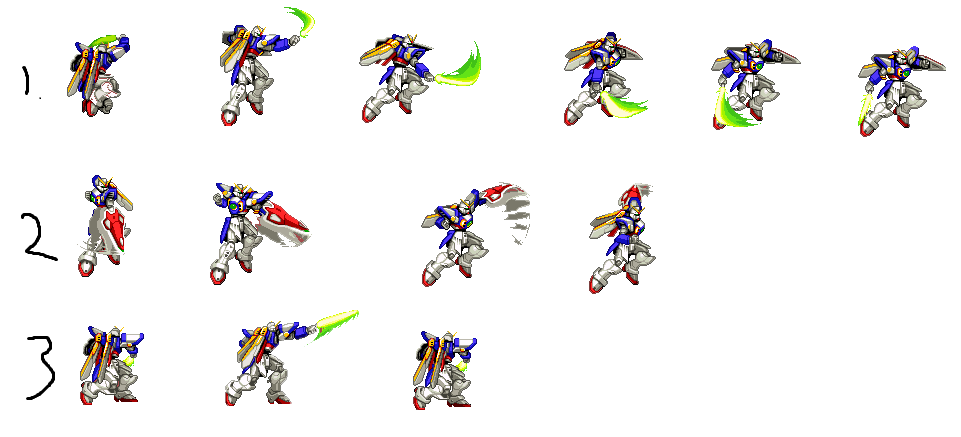
\includegraphics[width=0.8\textwidth]{airCombo.png} \\
        Below  is the planned attack data for each air attack \\
        
        airAttack1  
        \begin{enumerate}[noitemsep,nolistsep] 	 
        	\item attackDamage = 3
        	\item attackCollider = airAttack1 
        	\item startDelayTime  = 0.3f
        	\item durationTime = 0.5f
        	\item knockBackForce = zero
        	\item hitStunTime = 1
        	\item animationTrigger = "AirAttack1"
        	\item attackSound = "Air Swing"
        	\item cancelTime = 0.3f
        \end{enumerate} 
                airAttack2  
                \begin{enumerate}[noitemsep,nolistsep] 	 
                	\item attackDamage = 2
                	\item attackCollider = airAttack2 
                	\item startDelayTime  = 0.3f
                	\item durationTime = 0.6f
                	\item knockBackForce = zero
                	\item hitStunTime = 1
                	\item animationTrigger = "AirAttack2"
                	\item attackSound = "Air Swing2"
                	\item cancelTime = 0.3f
                \end{enumerate} 
        airAttack3 
         \begin{enumerate}[noitemsep,nolistsep] 	 
        	\item attackDamage = 5
        	\item attackCollider = airAttack3 
        	\item startDelayTime  = 0.3f
        	\item durationTime = 0.5f
        	\item knockBackForce = 300f
        	\item hitStunTime = 1
        	\item animationTrigger = "AirAttack3"
        	\item attackSound = "Air Swing3"
        	\item cancelTime = 0.3f
        	\end{enumerate} 
\subsubsection*{Level Fades}
there will be Texture2D called the fadeOutTexture which will be a black.png that will cover the player's camer. There will be a function that begins fade which will accept an int for direction. 1 being fade in and -1 being fade out. Begin fade will slowly increase or decrease the opacity of the black texture.
\subsubsection*{Save Progression}
There will be a save block that the user hits in order to save. There will always be one in the Boss walkway 
\subsubsection*{Player Re spawn Introduction}
The base jabber will be instantiated off the camera than enter the scene from the left side and than out through the ride side. When the base jabber x positions is above the re spawn point the GW will jump off the base jabber and land on the platform once the player has landed on the platform. The player gains control over GW.



        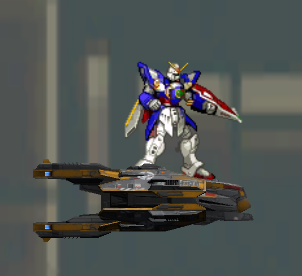
\includegraphics[width=0.8\textwidth]{baseJabber.png} \\
        the player on a base jabber



\subsubsection*{Enemy Tweaks}
Enemy GE will have a preAttack animation state and a end attack animation state. There transitions will be through triggers.


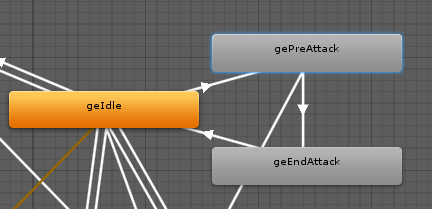
\includegraphics[width=0.8\textwidth]{preAnimation.png}

\subsubsection*{New Level}

Here is a sketch of the intended level for level 2 \\
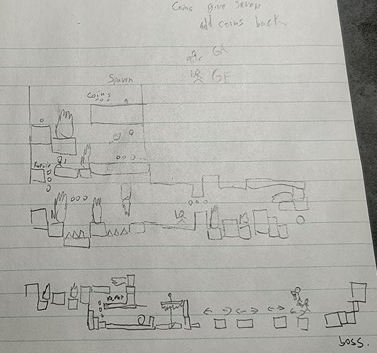
\includegraphics[width=0.8\textwidth]{level2.png} \\

\subsection*{Project Timeline}
This section only contains one chart for the project time line. Please refer to ProjectTime.xlsx for more charts, the complete timeline and responsibilities. \\
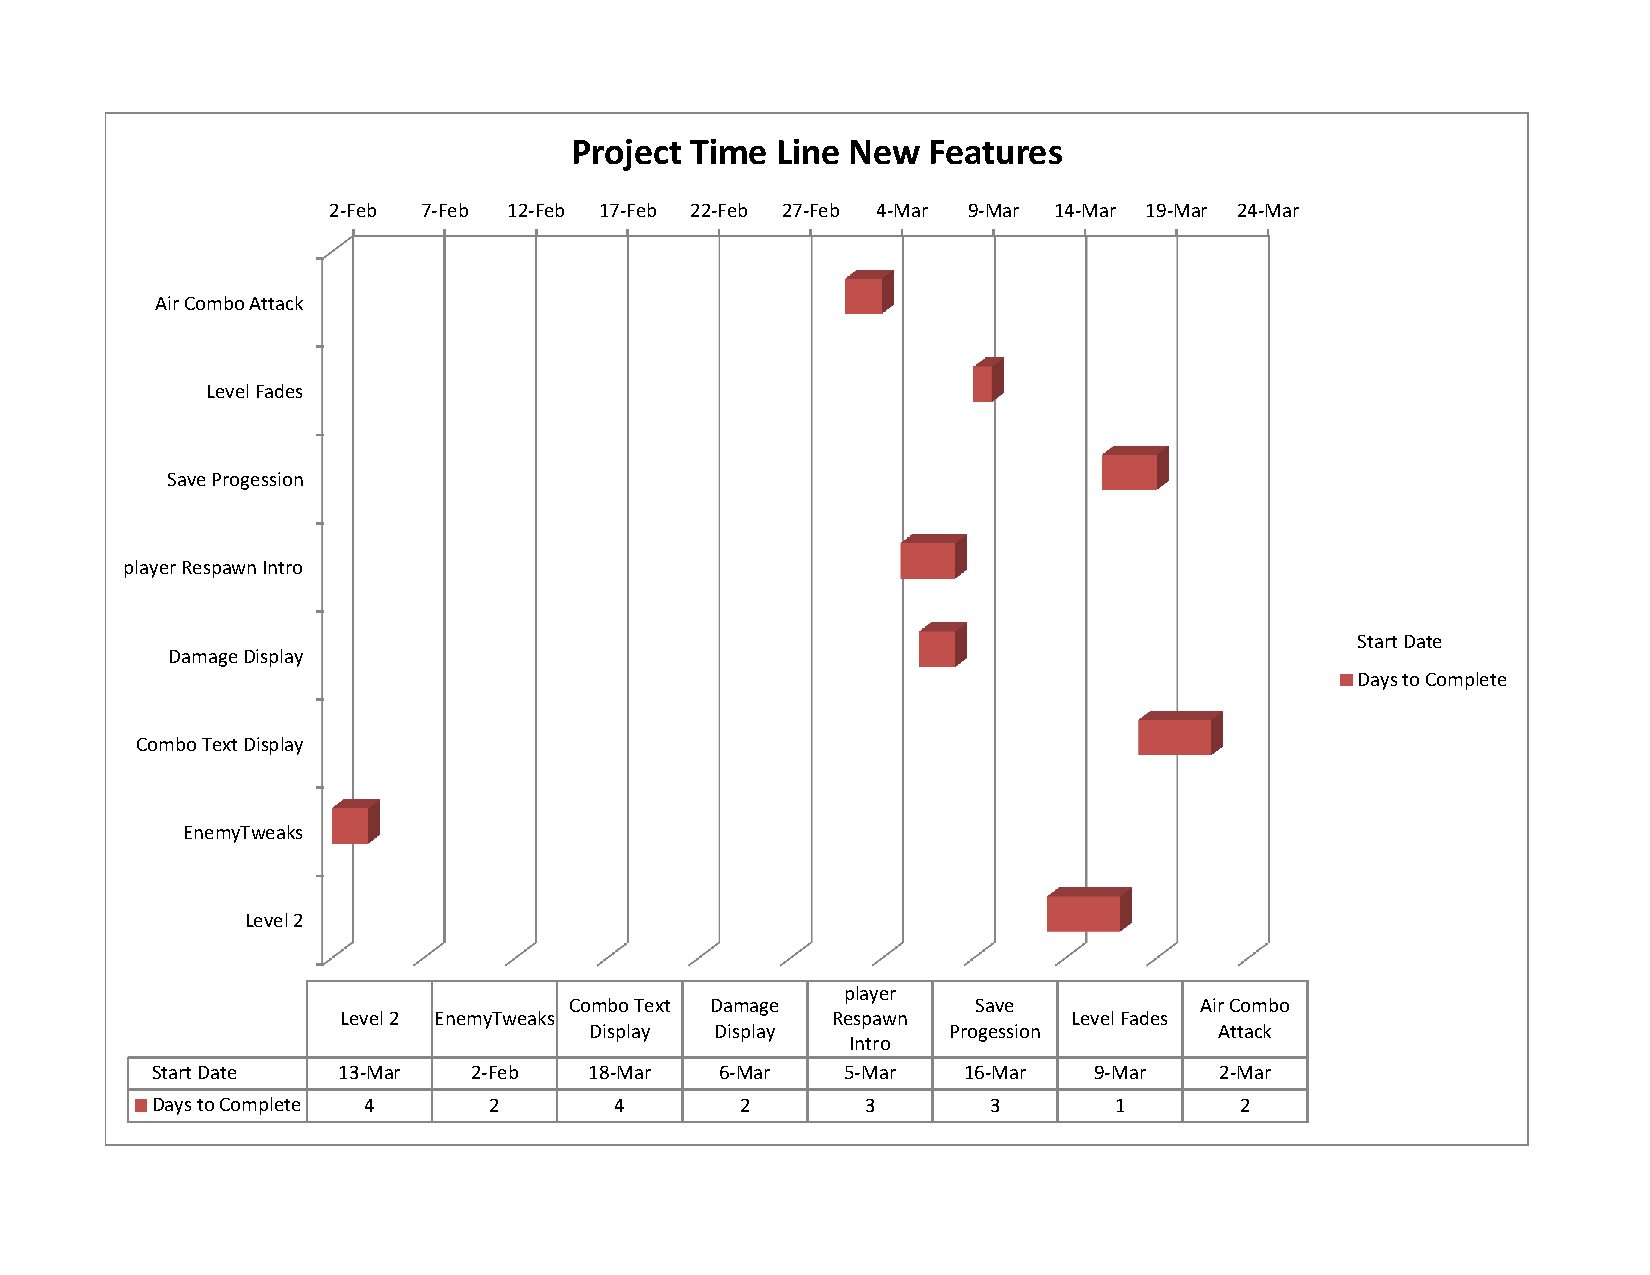
\includegraphics[width=0.8\textwidth]{ProjectTime.pdf} \\
\end{document}
